\section{Results}
\label{sec:results}

All eight members are scored on a common interval, 8 to 10 July 2025, which is
the intersection of the members' post-spinup spans and which contains the whole
drifter record. Members are coded by wave coupling (W), seagrass canopy (V) and
mobile bed (M). The attribution rests on the four fixed-bed members, and the
mobile-bed arm is reported beside them in the tables and examined in
Section~\ref{sec:res_sensitivity}.

\subsection{Water level}
\label{sec:res_wl}

Table~\ref{tab:wl} reports water level skill at the three interior stations.
Raw error is dominated by a positive bias at BocaNord and AltaVilaEst, between
0.03 and 0.09~m, and by a negative one at BocaSud, between $-0.051$ and
$-0.015$~m. The bias is a datum and boundary-offset property that all members
share and it is not what distinguishes them.

The anomaly RMSE responds to different factors at the three stations
(Figure~\ref{fig:wl}b). At BocaSud it varies by 1.6~mm across the four
fixed-bed members. At BocaNord it varies by 12~mm and follows wave coupling,
falling from 0.039 to 0.027~m without a canopy and from 0.038 to 0.031~m with
one. At AltaVilaEst, the innermost station, in the northern basin where the meadow
is densest, it varies by 32~mm and follows the canopy, the two
vegetated members giving 0.021 and 0.028~m with correlations of 0.94 and 0.95
and the two bare members 0.048 and 0.054~m with correlations of 0.79 and 0.81.
Modelled-to-observed standard deviation ratios move the same way, from 1.18 and
1.37 without a canopy to 1.01 and 1.18 with one. The mobile-bed members
reproduce the values of their fixed-bed counterparts to within 3~mm, with one
exception, the bare wave-coupled member at AltaVilaEst, whose anomaly RMSE is
8~mm lower than on the fixed bed and remains 16~mm above that of its vegetated
counterpart.

The record itself shows where that error sits (Figure~\ref{fig:wl}a), with the
bare configurations overshooting the range of the observed anomaly and running
ahead of it, most visibly on the falling limb of 9 July, while the vegetated
ones track both the amplitude and the phase. The two arms are separated by more
than the spread within either of them over most of the window.

\begin{figure}[H]
  \centering
  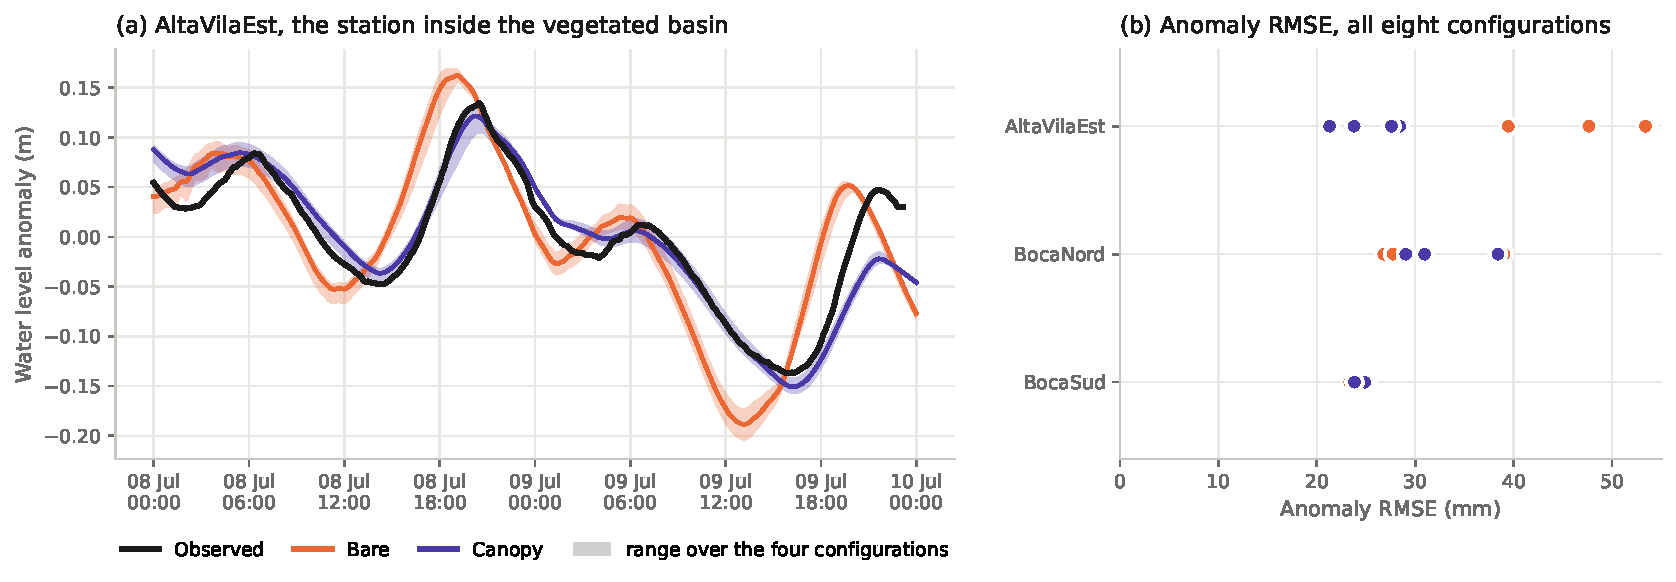
\includegraphics[width=\textwidth]{water_level_stations}
  \caption{Water level over the scored window. (a) Anomaly at AltaVilaEst,
  observed against the two arms, each drawn as its mean and the envelope of its
  four configurations, the mobile-bed ones included. Anomalies rather than raw
  levels, because the bias is common to all eight members. (b) Anomaly RMSE at
  the three stations for every configuration, coloured by canopy treatment.}
  \label{fig:wl}
\end{figure}

The vegetated members are three-day segments restarted from the bare member of
the same cell, and a segment run without any other change reproduces its
continuous member in water level and drifter skill (Supplementary Material,
Section~S7), so the separation at AltaVilaEst does not reflect the restart.

\begin{table}[H]
  \centering
  \caption{Water level skill by member and station, 8--10 July 2025.
  $\mathrm{RMSE}^2 = \mathrm{bias}^2 + \mathrm{RMSE}_{\mathrm{anom}}^2$. Members
  are coded by wave coupling (W), seagrass canopy (V) and mobile bed (M); the
  last four of each station form the mobile-bed arm. All values in metres
  except the dimensionless ratios.}
  \label{tab:wl}
  \begin{tabular}{llrrrrr}
    \toprule
    Station & Member & RMSE & Bias & RMSE$_{\mathrm{anom}}$ & $r$ & $\sigma_m/\sigma_o$ \\
    \midrule
    BocaNord & \texttt{{-}{-}{-}}  & 0.052 & $+0.035$ & 0.039 & 0.89 & 1.20 \\
             & \texttt{{-}V{-}}    & 0.050 & $+0.033$ & 0.038 & 0.90 & 1.22 \\
             & \texttt{W{-}{-}}    & 0.065 & $+0.059$ & 0.027 & 0.94 & 1.08 \\
             & \texttt{WV{-}}      & 0.059 & $+0.051$ & 0.031 & 0.92 & 1.09 \\
             & \texttt{{-}{-}M}    & 0.052 & $+0.034$ & 0.039 & 0.89 & 1.20 \\
             & \texttt{{-}VM}      & 0.050 & $+0.032$ & 0.038 & 0.90 & 1.22 \\
             & \texttt{W{-}M}      & 0.066 & $+0.060$ & 0.028 & 0.94 & 1.12 \\
             & \texttt{WVM}        & 0.059 & $+0.051$ & 0.029 & 0.94 & 1.15 \\
    \midrule
    BocaSud  & \texttt{{-}{-}{-}}  & 0.050 & $-0.043$ & 0.025 & 0.95 & 1.20 \\
             & \texttt{{-}V{-}}    & 0.057 & $-0.051$ & 0.025 & 0.95 & 1.16 \\
             & \texttt{W{-}{-}}    & 0.028 & $-0.015$ & 0.024 & 0.94 & 1.06 \\
             & \texttt{WV{-}}      & 0.035 & $-0.025$ & 0.025 & 0.93 & 1.02 \\
             & \texttt{{-}{-}M}    & 0.049 & $-0.043$ & 0.025 & 0.95 & 1.20 \\
             & \texttt{{-}VM}      & 0.057 & $-0.051$ & 0.025 & 0.95 & 1.16 \\
             & \texttt{W{-}M}      & 0.033 & $-0.023$ & 0.023 & 0.94 & 1.08 \\
             & \texttt{WVM}        & 0.037 & $-0.028$ & 0.024 & 0.93 & 1.05 \\
    \midrule
    AltaVila & \texttt{{-}{-}{-}}  & 0.076 & $+0.053$ & 0.054 & 0.81 & 1.37 \\
    Est      & \texttt{{-}V{-}}    & 0.049 & $+0.040$ & 0.028 & 0.94 & 1.18 \\
             & \texttt{W{-}{-}}    & 0.097 & $+0.085$ & 0.048 & 0.79 & 1.18 \\
             & \texttt{WV{-}}      & 0.070 & $+0.067$ & 0.021 & 0.95 & 1.01 \\
             & \texttt{{-}{-}M}    & 0.077 & $+0.055$ & 0.053 & 0.81 & 1.36 \\
             & \texttt{{-}VM}      & 0.050 & $+0.042$ & 0.028 & 0.94 & 1.17 \\
             & \texttt{W{-}M}      & 0.074 & $+0.062$ & 0.040 & 0.86 & 1.19 \\
             & \texttt{WVM}        & 0.062 & $+0.057$ & 0.024 & 0.94 & 1.01 \\
      \bottomrule
  \end{tabular}
\end{table}

\subsection{Lagrangian transport}
\label{sec:res_drifters}

Thirty-five drifters across twelve deployments were scored against each member
over the interval each drifter was in the water, which ranged from 0.4 to
7.2~hours. Table~\ref{tab:lagrangian} summarises the metrics and
Figure~\ref{fig:lagrangian} shows their distribution.

On the fixed bed, mean Liu--Weisberg skill spans 0.597 to 0.739 and endpoint
separation 327 to 481~m, and the four members divide cleanly on the canopy. The
two vegetated members score 0.711 and 0.739 and the two bare ones 0.597 and
0.619, and the two pairs do not overlap. The two components of the trajectory
error move together and both improve with the canopy, path length ratio rising
from 0.80 and 0.83 without a canopy to 0.88 and 0.94 with one, and mean heading
error falling from 11.2 and 10.4$^\circ$ to 8.5 and 8.4$^\circ$.

\begin{table}[H]
  \centering
  \caption{Lagrangian metrics by ensemble member, 35 drifters over twelve
  deployments, scored on the interval each drifter was in the water. Path ratio
  is simulated over observed path length. Heading error is the mean angular
  difference between simulated and observed step directions and is computed on
  eleven deployments, deployment 4 having too few positions to form the three
  step bearings it requires. The lower block is the mobile-bed arm
  (Section~\ref{sec:res_sensitivity}).}
  \label{tab:lagrangian}
  \begin{tabular}{lccrrrr}
    \toprule
    Member & Waves & Canopy & LW skill & Endpoint (m) & Path & Heading \\
    \midrule
    \texttt{{-}{-}{-}} & no  & no  & 0.619 & 478 & 0.80 & 11.2$^\circ$ \\
    \texttt{{-}V{-}}   & no  & yes & \textbf{0.739} & \textbf{327} & 0.88 & 8.5$^\circ$ \\
    \texttt{W{-}{-}}   & yes & no  & 0.597 & 481 & 0.83 & 10.4$^\circ$ \\
    \texttt{WV{-}}     & yes & yes & 0.711 & 335 & \textbf{0.94} & \textbf{8.4}$^\circ$ \\
    \midrule
    \multicolumn{7}{l}{\textit{Mobile bed}} \\
    \texttt{{-}{-}M}   & no  & no  & 0.614 & 479 & 0.80 & 11.4$^\circ$ \\
    \texttt{{-}VM}     & no  & yes & 0.739 & 330 & 0.88 & 8.5$^\circ$ \\
    \texttt{W{-}M}     & yes & no  & 0.708 & 304 & 0.89 & 7.9$^\circ$ \\
    \texttt{WVM}       & yes & yes & 0.718 & 307 & 0.88 & 8.0$^\circ$ \\
    \bottomrule
  \end{tabular}
\end{table}

\begin{figure}[H]
  \centering
  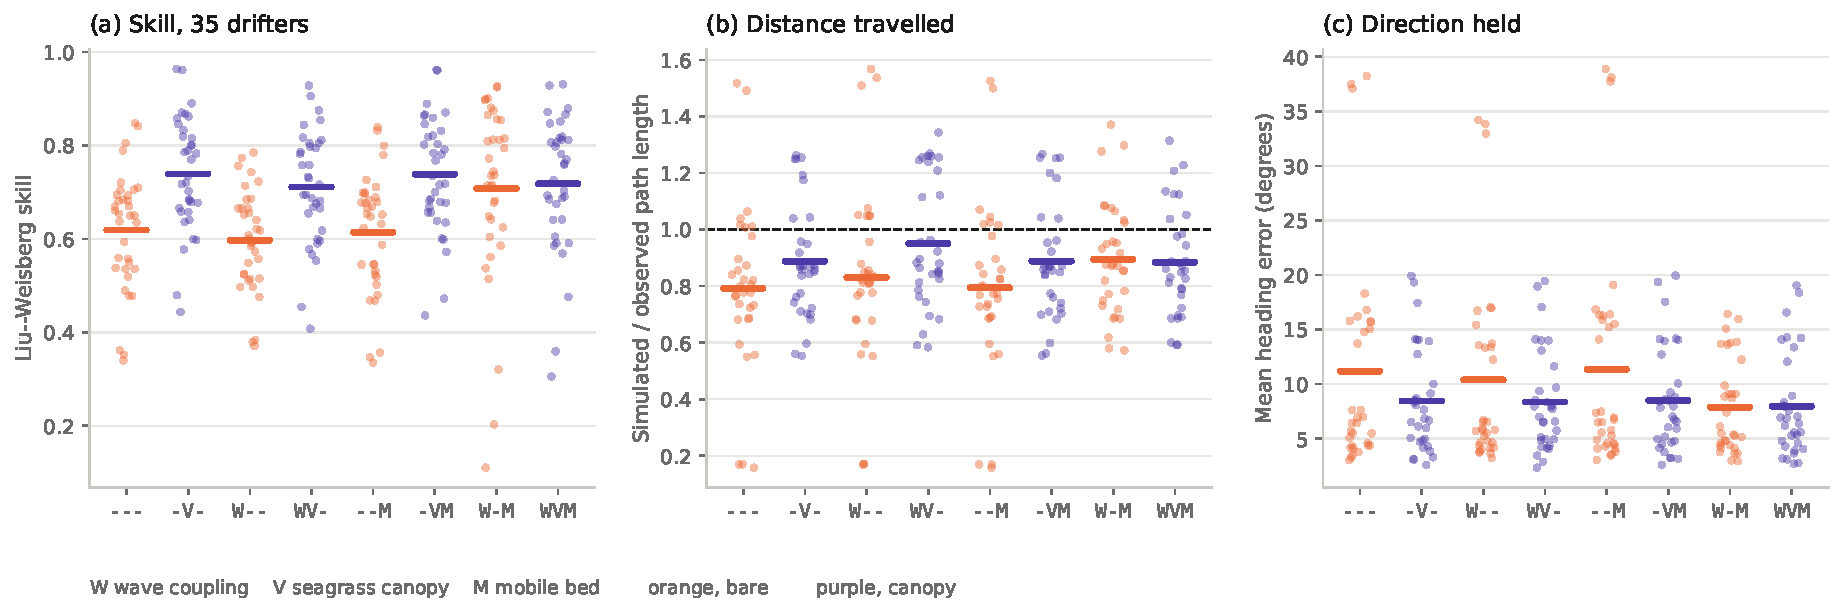
\includegraphics[width=\textwidth]{lagrangian_results}
  \caption{Lagrangian validation, one point per drifter and the bar giving the
  mean, the four fixed-bed members on the left and the mobile-bed arm on the
  right. (a) Liu--Weisberg skill. (b) Simulated over observed path length, the
  dashed line marking equality. (c) Mean angular difference between simulated
  and observed step directions. Panels (b) and (c) carry 32 drifters rather than
  35, deployment 4 having too few positions to form step bearings.}
  \label{fig:lagrangian}
\end{figure}

Figure~\ref{fig:tracks} shows the tracks for every deployment and for the
wave-coupled fixed-bed pair that differs only in the canopy. In the central
basin the bare particles leave the observed path early and finish short of the
observed endpoint while the vegetated ones hold its heading, and in the
southern deployments both follow the observed path closely, deployment 4 being
the exception.

\begin{figure}[H]
  \centering
  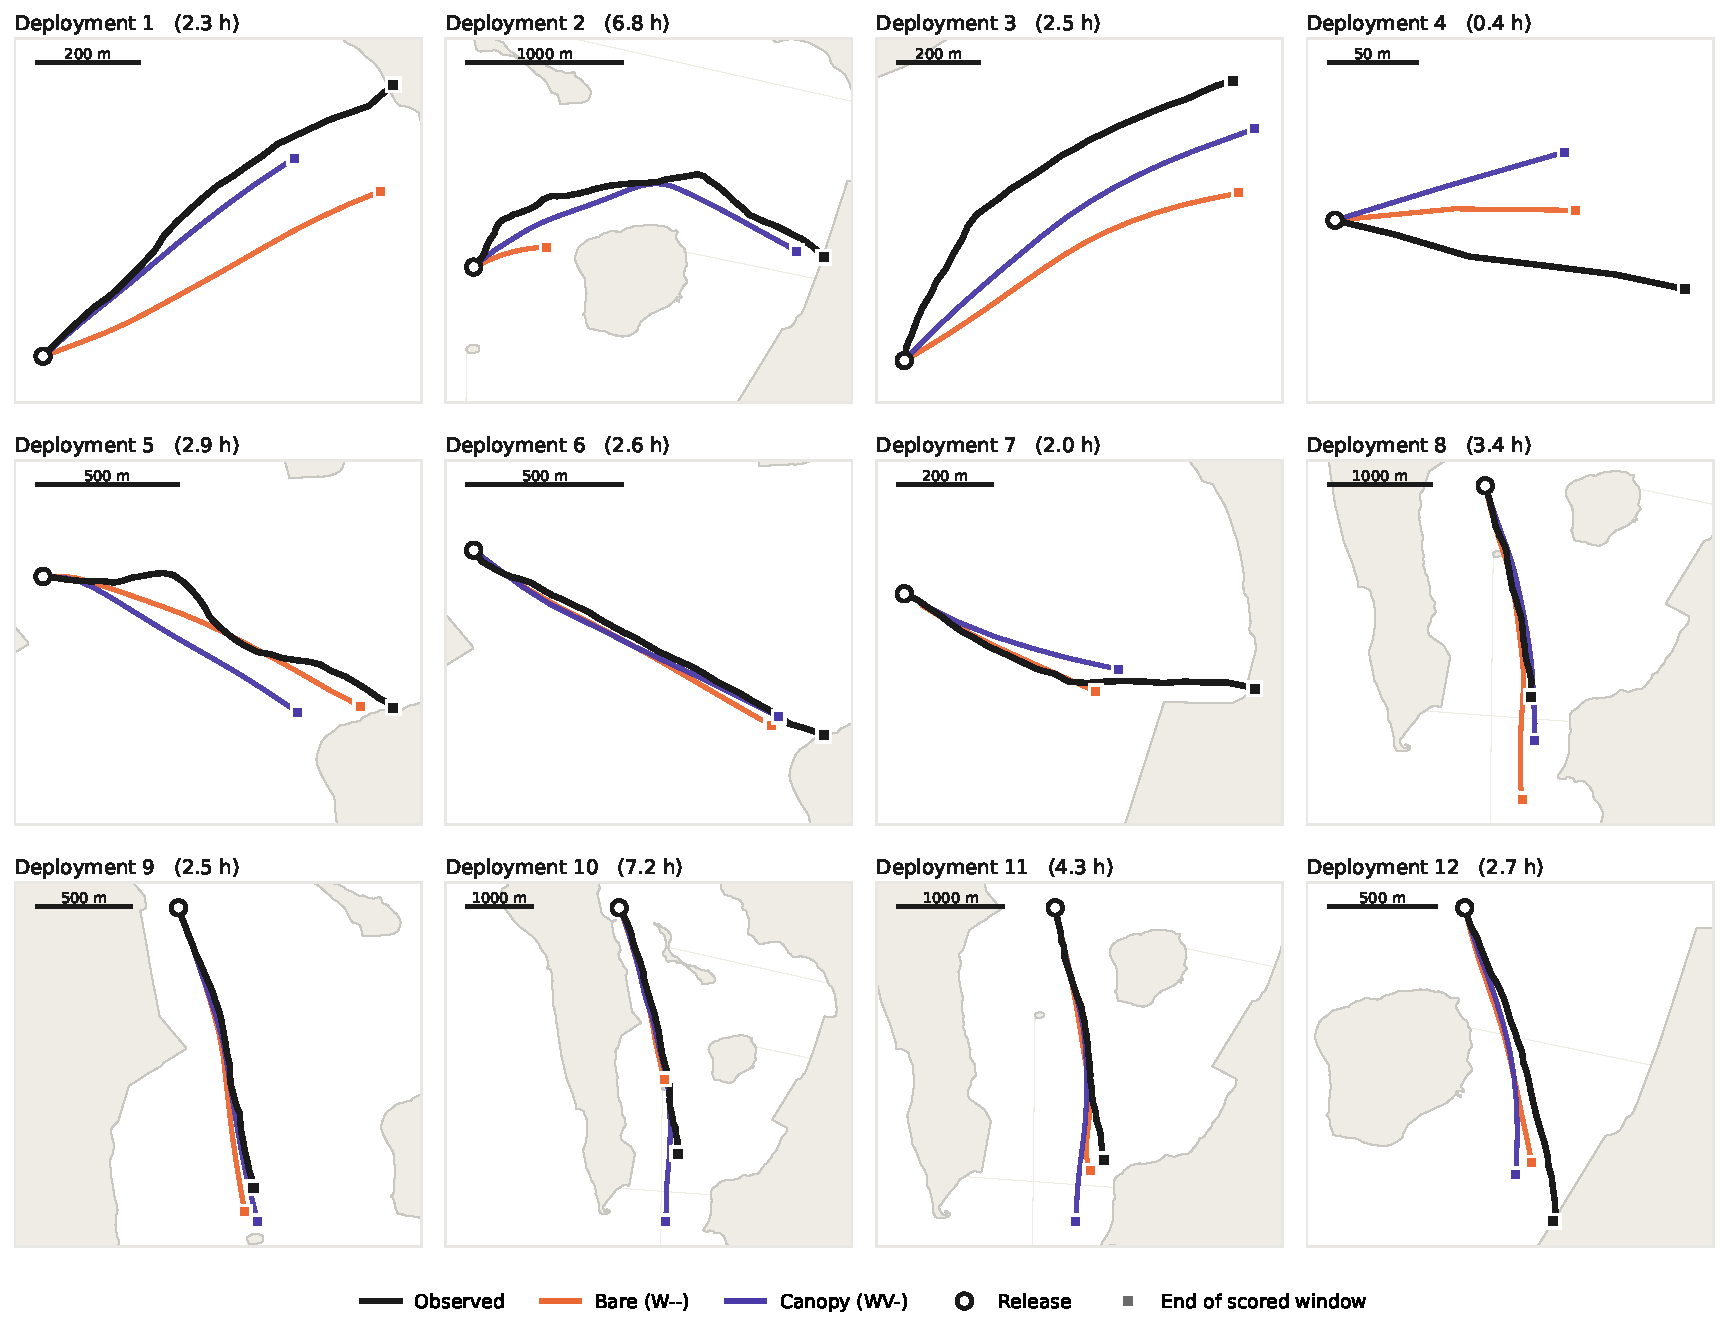
\includegraphics[width=\textwidth]{drifter_trajectories}
  \caption{Observed and simulated drifter trajectories, all twelve deployments,
  for the wave-coupled fixed-bed configurations that differ only in the canopy.
  One drifter per panel, the median-skill drifter of its deployment under the
  vegetated configuration. Circles mark the release and squares the end of the
  scored window. Each track is clipped to the interval its drifter was in the
  water. Panel extents differ, so each carries its own scale bar.}
  \label{fig:tracks}
\end{figure}

\subsection{Process attribution}
\label{sec:res_attribution}

On the fixed bed the design is a two-factor factorial in wave coupling and
canopy, with two single-factor contrasts per factor.
Figure~\ref{fig:attribution} gives them, with the contrasts that involve the
mobile bed beside them, with bootstrap confidence intervals over 4000 paired
resamples.

\textbf{Canopy.} The canopy raises skill by 0.120 (95\% CI $+0.061$ to $+0.180$)
without waves and by 0.114 (CI $+0.056$ to $+0.170$) with them, with 25 and 27
of the 35 drifters improving. Both intervals are clear of zero, and the two
contrasts agree to within 0.006, so the canopy effect does not depend on the
wave treatment.

\textbf{Wave coupling.} Wave coupling reduces skill by 0.022 (CI $-0.043$ to
$-0.003$) without a canopy and by 0.028 (CI $-0.040$ to $-0.017$) with one,
with 21 and 25 of the 35 drifters worse. The effect is a fifth of that of the
canopy, and the interaction term of the two factors is $-0.006$.

The canopy contrast holds deployment by deployment (Figure~\ref{fig:attribution}b),
with the same sign under both wave treatments in ten of the twelve deployments.
Deployment 4, the shortest record and the one deployment in which the bare
members score higher, is retained, and excluding it widens the two canopy
contrasts to $+0.148$ and $+0.144$ (Section~S7).

\begin{figure}[H]
  \centering
  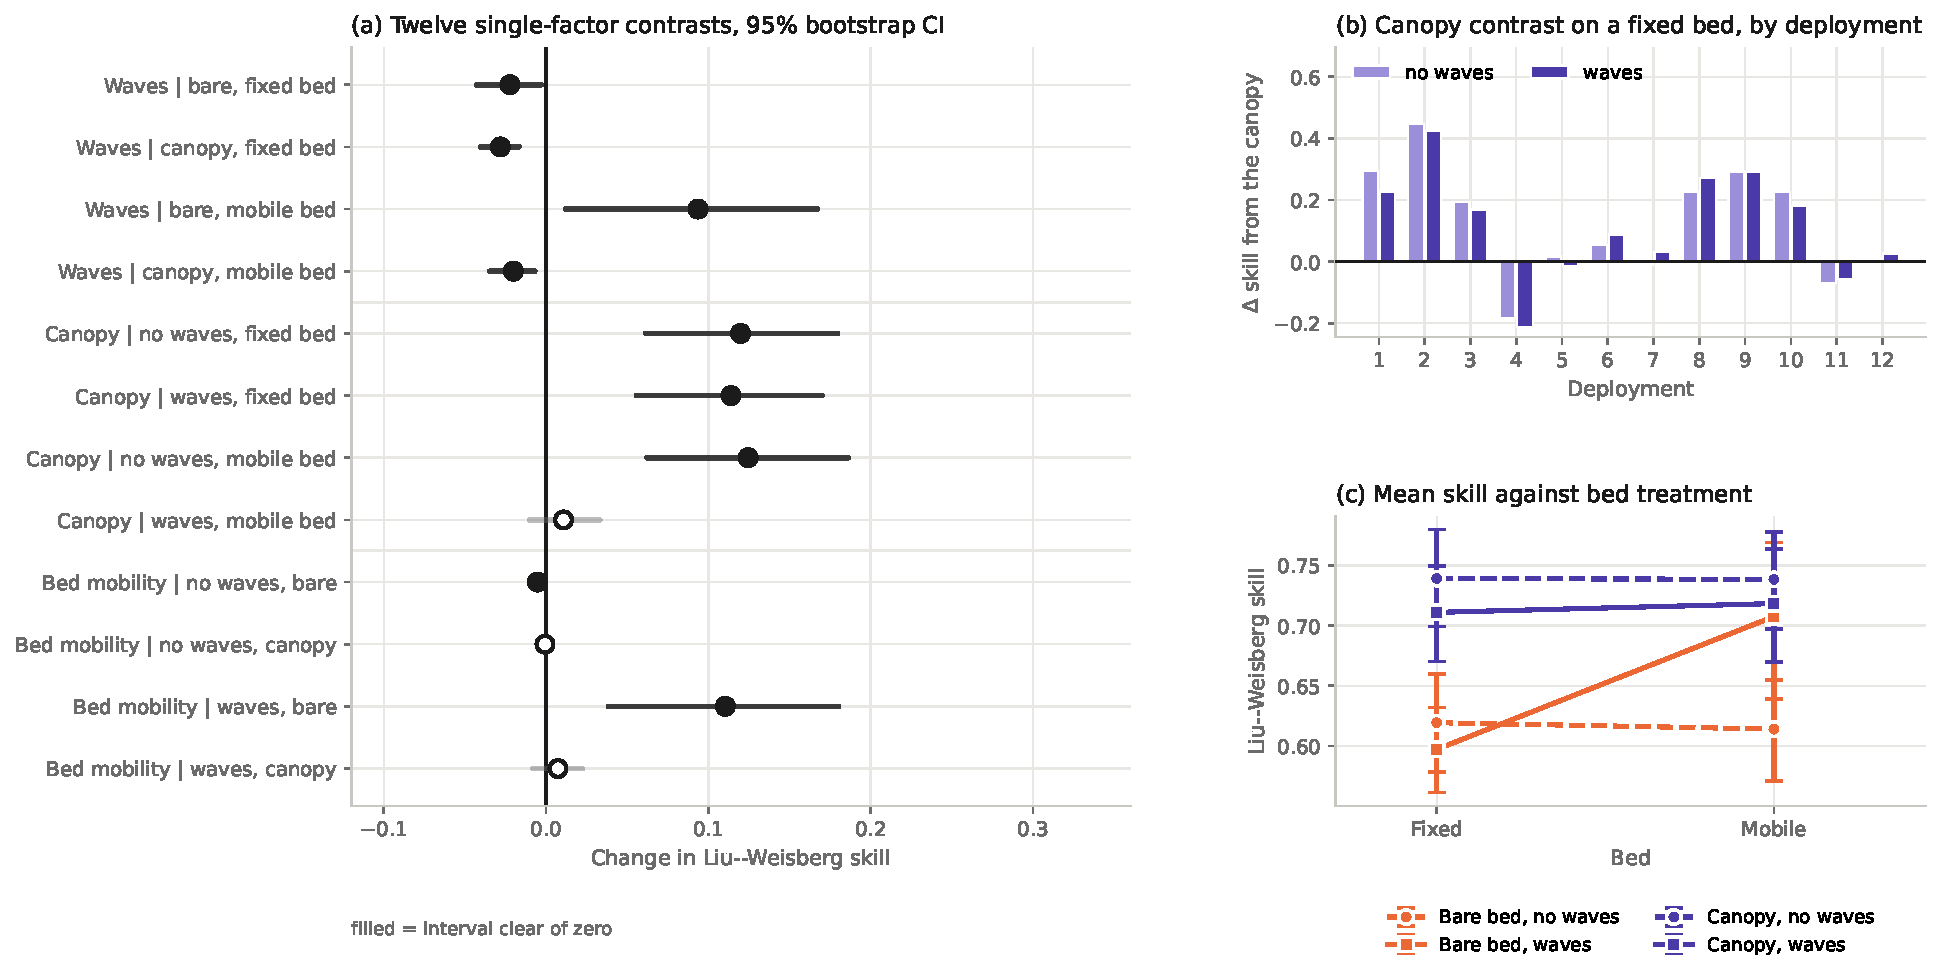
\includegraphics[width=\textwidth]{ensemble_attribution}
  \caption{Process attribution. (a) The twelve single-factor contrasts of the
  three-factor design with 95\% bootstrap intervals over 4000 paired resamples,
  filled markers denoting intervals clear of zero; the contrasts involving the
  mobile bed belong to the sensitivity arm. (b) The canopy contrast on the
  fixed bed, deployment by deployment, without and with wave coupling. (c) Mean
  skill against bed treatment, one line per combination of canopy and wave
  treatment, with 95\% intervals on each mean.}
  \label{fig:attribution}
\end{figure}

\subsection{Three-dimensional structure}
\label{sec:res_3d}

Over the wet cells of the lagoon interior, with the inlets excluded, mean
current speed increases monotonically from the bed to the surface in every
member (Figure~\ref{fig:profile}), and the canopy sets the shape of that
profile. On the fixed bed without a canopy, bed-layer speed is 0.032 to
0.035~\si{\metre\per\second} and surface-layer speed 0.065 to
0.069~\si{\metre\per\second}, for surface-to-bed ratios of 1.88 and 2.14. With a
canopy, bed-layer speed falls to 0.0093 to 0.0095~\si{\metre\per\second} while
surface speed falls much less, to 0.043 to 0.047~\si{\metre\per\second}, and the
ratio rises to 4.50 and 5.05.

Wave coupling moves the ratio by far less, adding 0.26 in the bare arm and 0.55
in the vegetated one, against a canopy contribution of $+2.62$ without waves and
$+2.91$ with them.

Bed shear stress separates the two treatments by sign rather than by magnitude.
Averaged over the meadow on 8 July in members started from the stratified
column, as the ensemble is, it fell from 0.028 to 0.0026~\si{\pascal} when the
canopy was introduced, a factor of 11, while a member representing the same
meadow as an equivalent bed roughness instead of as a canopy raised it to
0.043~\si{\pascal} over the same cells and times.

Lagoon-mean surface speed does not order the members the way transport does,
since the member reproducing the observed drifter behaviour best has the lowest
lagoon-mean surface speed of the fixed-bed members at
0.043~\si{\metre\per\second}, against 0.069 for a member whose particles travel
17\% too short a distance.

\begin{figure}[H]
  \centering
  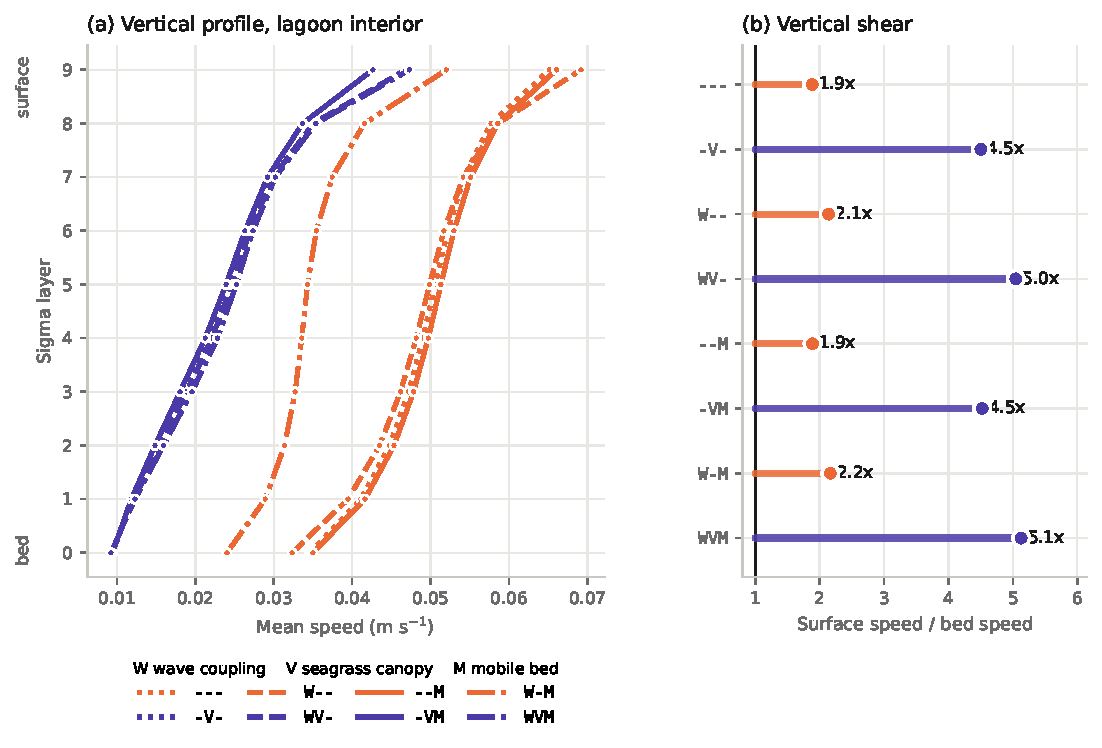
\includegraphics[width=0.88\textwidth]{layer_profile_lagoon}
  \caption{Vertical structure in the lagoon interior over the drifter window.
  (a) Mean speed by sigma layer, colour giving the canopy treatment and line
  style the wave and bed treatments. (b) The ratio of surface to bed speed.}
  \label{fig:profile}
\end{figure}

\subsection{Response of the seagrass classes}
\label{sec:res_classes}

Cells were grouped by the seagrass class of the nearest classified point. The
classes occupy different parts of the basin at different depths, and the bare
fixed-bed configurations already have their \emph{Posidonia} cells slower at
the bed than their sand cells, in a ratio of 0.91 and 0.92, so the canopy
effect is read between configurations within a class or as a change in that
ratio.

Under either reading the effect is large and correctly ordered, since on the
fixed bed introducing the canopy reduces mean bed speed by 78\% over
\emph{Posidonia} and 77\% over \emph{Cymodocea}, against 59\% over sand and 57\%
over rock (Figure~\ref{fig:classes}b). The \emph{Posidonia} to sand bed-speed
ratio falls from 0.91 and 0.92 without a canopy to 0.49 with one, under both
wave treatments. The two unvegetated classes respond as well, because slowing
the flow through the meadow changes the circulation of a basin whose interior
is largely meadow, but they respond by a quarter less.

The canopy also removes most of the dependence on wave coupling, since within a
class mean bed speed differs between the two bare fixed-bed configurations by
0.002 to 0.010~\si{\metre\per\second} and between the two vegetated ones by
0.0002 to 0.0011~\si{\metre\per\second}. Once the canopy is present the near-bed
flow is nearly the same whatever the wave treatment, which is the near-bed
counterpart of the agreement in transport skill reported in
Section~\ref{sec:res_drifters}.

The wave field does not follow the flow, mean orbital velocity at the bed
changing by 0.2 to 0.9\% over the four classes when the canopy is introduced on
the fixed bed (Figure~\ref{fig:classes}c), since the canopy does not reach the
wave computation (Section~\ref{sec:disc_limits}).

\begin{figure}[H]
  \centering
  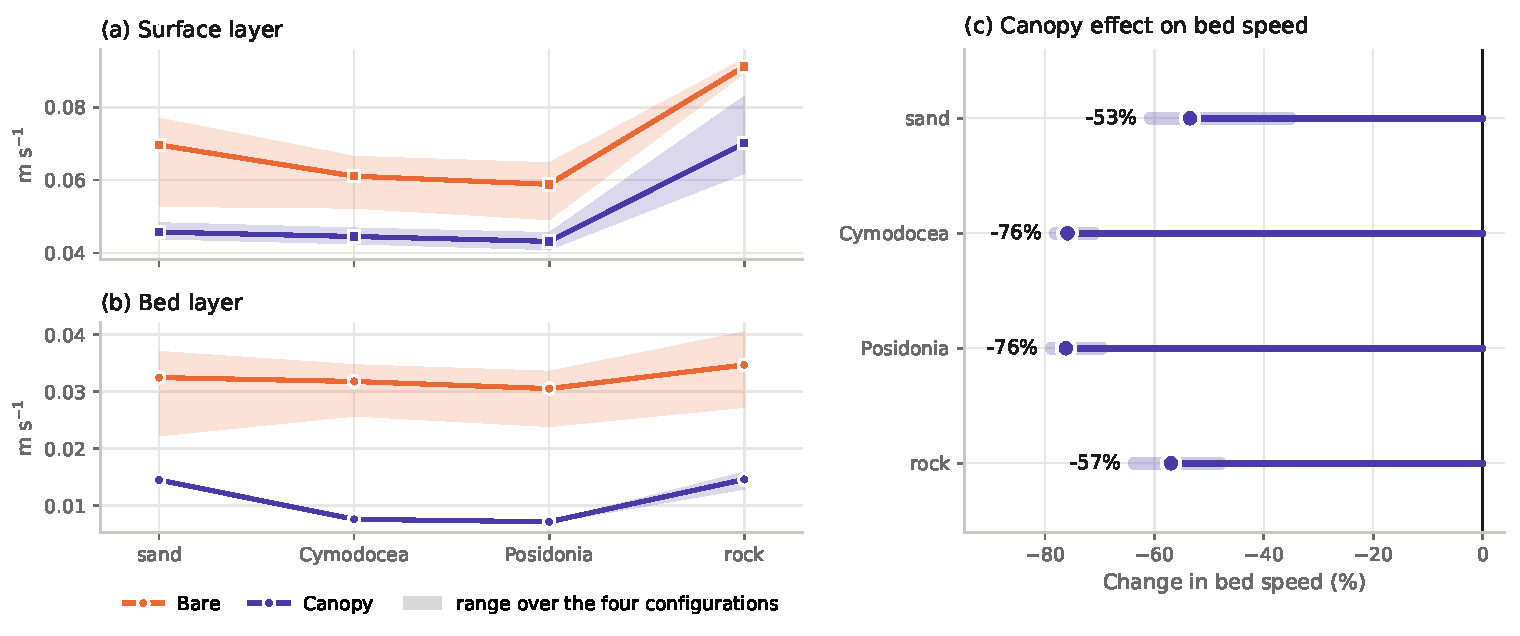
\includegraphics[width=\textwidth]{class_speed_uorb}
  \caption{Flow response by seagrass class in the lagoon interior. (a) Mean
  speed in the surface layer and (b) in the bed layer, the line giving the mean
  over the four configurations of each arm, the mobile-bed ones included, and
  the band their range. (c) Change in mean bed speed on introducing the canopy,
  the marker giving the mean over the four cells of the design and the band
  their range.}
  \label{fig:classes}
\end{figure}

\subsection{Sensitivity to bed mobility, initial condition and discretisation}
\label{sec:res_sensitivity}
\label{sec:res_numerics}

With wave coupling the mobile bed leaves any plausible state of the basin.
Averaged over the lagoon from 7 to 10 July, suspended sediment reaches
9.3~\si{\gram\per\litre} in the bare wave-coupled member and
9.4~\si{\gram\per\litre} in its vegetated counterpart, against 0.1 and
0.007~\si{\gram\per\litre} in the two uncoupled mobile-bed members, and the bed
of the lagoon loses 4.0 and 3.1~million~\si{\metre\cubed} over the nine days.
By 10 July the bare wave-coupled member has lowered the lagoon bed by 12~cm on
average and changed it by more than 5~cm over 74\% of its area, whereas without
waves the change exceeds 5~cm over 0.3\% of the area. The canopy does not
shield the bed from this erosion, because it does not reach the wave model.

The same bare member nevertheless scores 0.708 (Table~\ref{tab:lagrangian}),
close to the vegetated members, so that in the cell combining waves and a
mobile bed the canopy contrast falls to $+0.011$ (CI $-0.010$ to $+0.033$) and
the wave and bed-mobility contrasts of the bare arm reach $+0.094$ and $+0.111$
(Figure~\ref{fig:attribution}a). The two segments restarted on 7~July locate
the source of that skill. With the bed updated the segment scores 0.710 and
with the bed held at its 7~July state 0.707, a difference of $-0.003 \pm
0.004$, while the held bed scores $0.110 \pm 0.039$ above the fixed-bed member
\texttt{W{-}{-}}, with 29 of 35 drifters better. The gain therefore comes from
the bathymetry reshaped over the first six days and not from sediment transport
in the drifter window. At AltaVilaEst the member keeps an anomaly RMSE of
0.040~m and a correlation of 0.86, against 0.024~m and 0.94 for its vegetated
counterpart.

Started from a vertically uniform column instead of the stratified state, the
bare members score 0.080 to 0.145 lower and the vegetated members 0.005 to
0.018 lower, so that the canopy contrasts on the fixed bed become $+0.195$ and
$+0.188$. The uniform start raises the modelled mean water level at the gauges
by 2 to 10~cm and, on the fixed bed, changes anomaly RMSE by at most 4~mm and
correlation by at most 0.03, and the canopy signature at AltaVilaEst is the same
under both starts.

The horizontal and vertical resolution, the time-step limit and the host and
decomposition change skill by less than 0.01 under a Courant limit of 0.5 and
water level by at most 2.4~mm, so they do not limit the quantities the study
reports (Section~S6). Under the Courant limit of 0.7 used by the ensemble the
uncoupled member scores $0.034 \pm 0.004$ lower on four partitions on a second
computer than on eight on the server, a dependence that all members share.

